\documentclass{article}
\usepackage[utf8]{inputenc}
\usepackage[english]{babel}
\usepackage[font=small,labelfont=bf]{caption}
\usepackage{geometry}
\usepackage{natbib}
\usepackage{pxfonts}
\usepackage{graphicx}
\usepackage{newfloat}
\usepackage{setspace}
\usepackage{hyperref}
\usepackage{placeins}

\newcommand{\argmax}{\mathop{\mathrm{argmax}}\limits}
\newcommand{\argmin}{\mathop{\mathrm{argmin}}\limits}

\newcommand{\methodsdemo}{1}
\newcommand{\topicprops}{2}
\newcommand{\listlearning}{3}
\newcommand{\precisiondistinctiveness}{4}
\newcommand{\precisiondistinctivenessdetail}{5}
\newcommand{\trajectories}{6}
\newcommand{\wordles}{7}
\newcommand{\brains}{8}


\title{\textit{Supporting Information for}: Geometric models reveal behavioral and neural signatures of transforming experiences into memories}
\author{Andrew C. Heusser\textsuperscript{1, 2, \textdagger}, Paxton C. Fitzpatrick\textsuperscript{1, \textdagger}, and Jeremy R. Manning\textsuperscript{1, *}\\\textsuperscript{1}Department of Psychological and Brain Sciences\\Dartmouth College, Hanover, NH 03755, USA\\\textsuperscript{2}Akili Interactive Labs\\Boston, MA 02110, USA\\\textsuperscript{\textdagger}Denotes equal contribution\\\textsuperscript{*}Corresponding author: Jeremy.R.Manning@Dartmouth.edu}

\bibliographystyle{apa}

\begin{document}

\renewcommand{\figurename}{Supplementary Figure}

%\begin{titlepage}
%  \maketitle
%  \thispagestyle{empty}
%\end{titlepage}

\setcounter{equation}{0}
\setcounter{figure}{0}
\setcounter{table}{0}
\setcounter{page}{1}
\setcounter{section}{0}
\makeatletter
%\renewcommand{\theequation}{S\arabic{equation}}
%\renewcommand{\thefigure}{S\arabic{figure}}
\renewcommand{\bibnumfmt}[1]{[S#1]}
\renewcommand{\citenumfont}[1]{S#1}


%\section*{Overview}
%This document provides additional details about the methods we used in the main text.  We also %include some additional analyses referenced in the main text.

\section*{Supplementary methods}
\subsection*{Optimizing topic model parameters}
In order to create accurate episode and recall models, we used an optimization method that was driven by our ability to explain hand-annotated memory performance metrics collected by \cite{ChenEtal17}.  In an earlier variant of our study~\citep{HeusMann18}, we used a grid search to compute the $\omega$ (episode sliding window duration, in scenes), $\rho$ (recall sliding window duration, in sentences), and $K$ (number of topics) that satisfied
\[
\argmax_{\omega, \rho, K} \left[\mathrm{corr}\left(\mathrm{corr}\left(\mu\left(\omega, \rho, K\right), \nu\left(\omega, \rho, K\right)\right), \theta\right)\right],
\]
where $\mathrm{corr}(\mu, \nu)$ is the per-participant correlation between the episode ($\mu$) and recall ($\nu$) topic proportions matrices, and $\theta$ is the per-participant hand-counted number of recalled scenes.  We searched over a grid of pre-specified values for each of these parameters; the resulting correlations are displayed in Supplementary Figure~\ref{fig:paramsearch}.  The optimal parameters were $\omega = 50$, $\rho = 10$, and $K = 100$.  In our current paper we made a number of improvements to how we preprocessed text and fit topic models (see \textit{Methods}), but we carried the same optimal parameters forward from \cite{HeusMann18} without performing any additional optimization.


\begin{figure}[b]
\centering
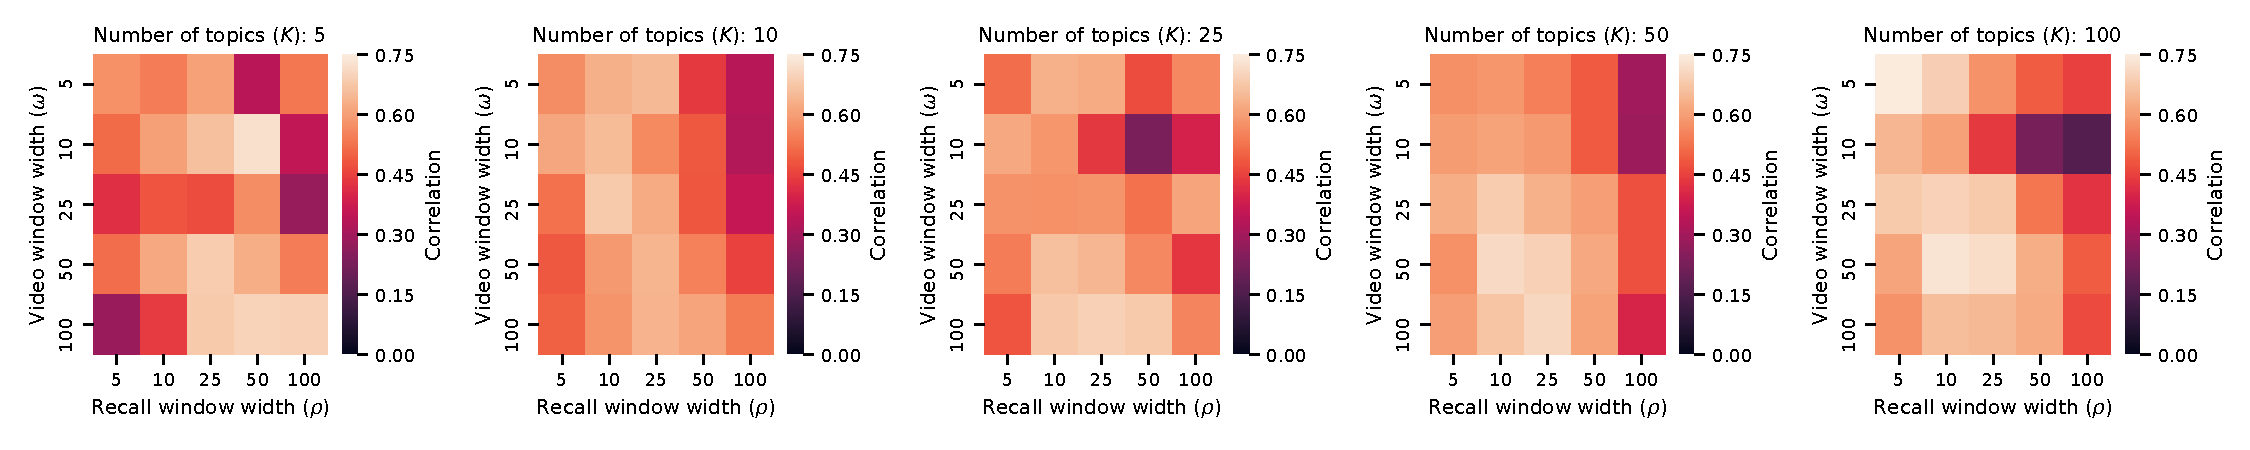
\includegraphics[width=1\textwidth]{figs/parameter_search}
\caption{\small \textbf{Optimizing topic model parameters.}  We performed a grid search over episode sliding window length ($\omega \in \{5, 10, 25, 50, 100 \}$), recall sliding window length ($\rho \in \{5, 10, 25, 50, 100 \}$), and number of topics ($K \in \{5, 10, 25, 50, 100 \}$).  The reported correlations are between per-participant episode-recall correlations and per-participant hand-counted numbers of recalled scenes.}
\label{fig:paramsearch}
\end{figure}

The optimized model converged on 32 unique topics that were assigned non-zero weights.  We provide a list of the top ten highest-weighted words from each topic in Supplementary Figure~\ref{fig:topics}.

\begin{figure}[p]
\centering
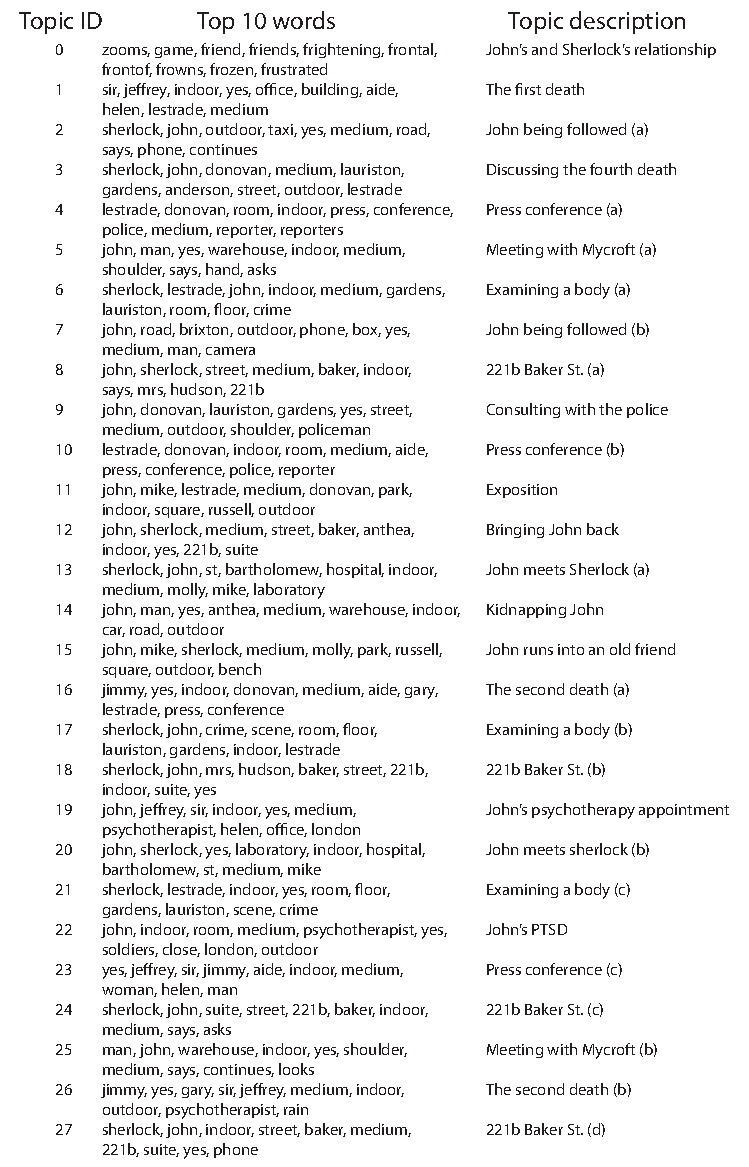
\includegraphics[width=0.65\textwidth]{figs/topic_words}
\caption{\small \textbf{Topics discovered in \textit{Sherlock}.} We applied a topic model to hand-annotated information about 1000 scenes spanning the 48-minute episode.  We identified 32 unique topics with non-zero weights (we used $K=100$ topics to fit the model).  Each topic comprises a distribution of weights over all words in the vocabulary.  For each topic, we show the words with the 10 largest weights, along with a suggested description of the topic.}
\label{fig:topics}
\end{figure}
%\FloatBarrier

\subsection*{Feature importance analyses}
To determine the contribution of each feature to the temporal structure of the episode topic proportions matrix, we conducted a ``leave one out'' analysis.  Specifically, we compared the original episode's topic proportions matrix (created using all hand-annotated features from the 998 manually identified scenes spanning the \textit{Sherlock} episode; see \textit{Methods} for a full list of features) with topic proportions matrices created using all but one type of feature.  For each impoverished topic proportions matrix, we computed the timepoint-by-timepoint correlation matrix, and correlated the proximal diagonals from the upper triangle with those from the temporal correlation matrix of the feature-complete matrix (for details on how we isolated proximal temporal correlations, see \textit{Methods}).  Observing a lower correlation between an impoverished matrix (with a particular feature removed) and the feature-complete matrix would suggest that the held-out feature contributed more prominently to the full episode topic proportion matrix's temporal structure.  We found that hand-annotated narrative details played the greatest roll in determining the temporal structure of the episode, whereas the name of the character(s) in focus for each shot contributed least (Supp. Fig.~\ref{fig:feature-importance}A).

\begin{figure}[]
\centering
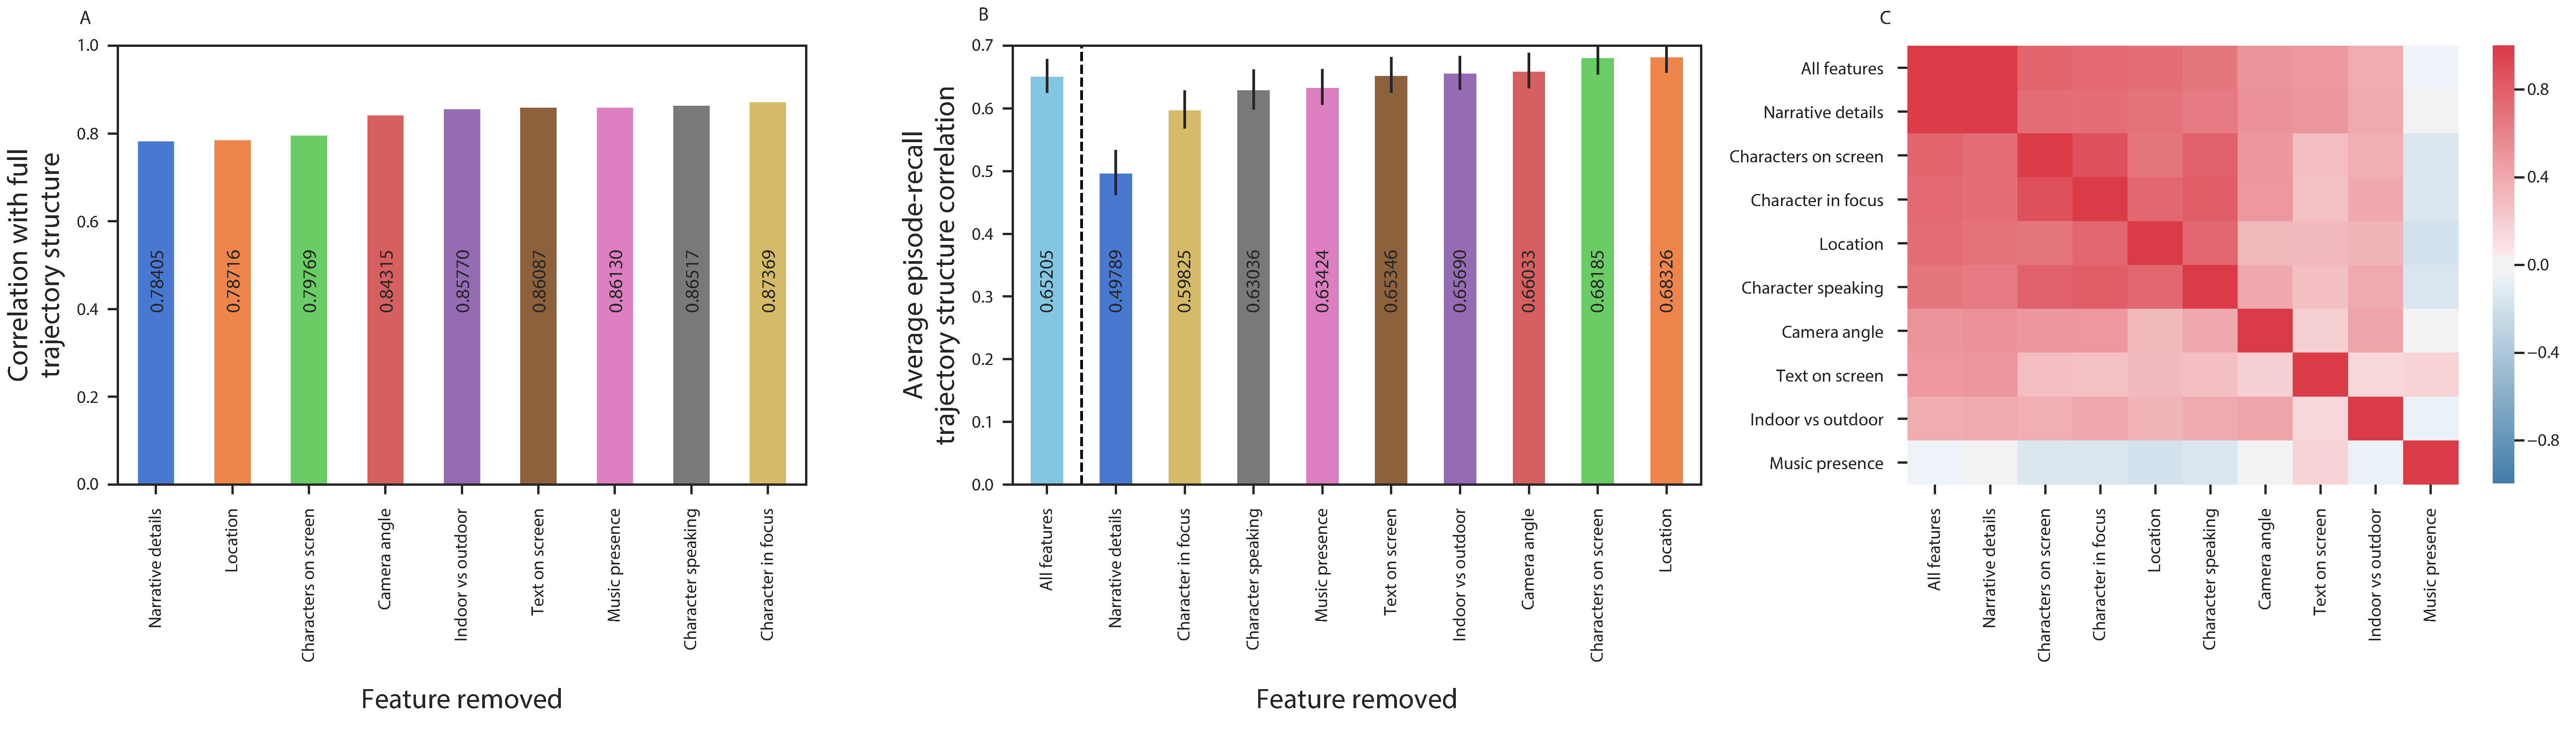
\includegraphics[width=1\textwidth]{figs/feature_value}
\caption{\small \textbf{Feature importance analysis.} \textbf{A.} Contributions of each feature type to the structure of the episode topic proportions matrix. The bar heights reflect the correlation between the proximal temporal structure (see \textit{Methods}) of the episode topic proportions matrix computed using all features, and that of an episode topic proportions matrix computed using all features except the indicated feature.  Lower bars reflect features that contribute more substantially to the episode's temporal structure. \textbf{B.} Which features are preserved during recall?  The bar heights reflect the (average) across-participant correlations between the proximal temporal structure of episode and recall topic proportions matrices constructed in the absence of the given feature.  Error bars denote standard error of the mean.  \textbf{C.} Feature correlation matrix.  Each entry displays the correlation between episode topic portions matrices created using only the indicated (row/column) features.}
\label{fig:feature-importance}
\end{figure}

Next, we sought to determine which annotated features contributed aspects of the episode's temporal structure that were preserved in participants' later recalls.  Specifically, we computed the timepoint-by-timepoint correlation matrix of the episode's topic proportions matrix, and correlated the proximal diagonals from its upper triangle with those from the timepoint-by-timepoint correlation matrices for each participant's recall topic proportions matrices (stretched via linear interpolation to have the same number of timepoints as the episode topic proportions matrix).  This yielded a single correlation coefficient for each participant.  We then repeated this analysis with each annotated feature held out in turn.  Observing a lower correlation between the episode and recall topic proportions matrices (constructed in the absence of a given feature) would indicate that participants utilize changes in that feature's content to discriminate between sections of the episode when organizing their recalls.  We found that hand-annotated narrative details were the most heavily utilized feature, whereas changes in the text present on-screen, the indoor/outdoor distinction between shots, the camera angle, the names of the various characters on screen, and the shot's location tended not to impact participants' recall structures (i.e., removing those features resulted in a \textit{greater} episode-recall correlation than including them; Supp. Fig.~\ref{fig:feature-importance}B).

We also wondered how the different types of features might relate.  For example, knowing which character is in focus during a given scene may also provide information about which character is speaking.  We computed topic proportions matrices from the annotations for each individual feature, in turn, and (using the same technique as in the above analyses) compared the proximal temporal correlation structure of each single-feature topic proportions matrix to each other, as well as to that of the full episode.  This provided additional confirmation that the full episode's temporal structure was largely driven by narrative details.  We also found that character-driven features (characters on screen, characters speaking, and characters in focus) were strongly correlated.  Other details, such as the presence or absence of music, led to very different topic proportions matrices (Supp. Fig.~\ref{fig:feature-importance}C).
%\FloatBarrier

\subsubsection*{Binary features}
Two categories of annotations, ``Music presence'' and ``Indoor vs outdoor,'' comprise a single word that can each take on one of two possible values (music: ``yes'' or ``no''; indoor vs outdoor: ``indoor'' or ``outdoor'').  Participants are unlikely to use the words ``yes'' or ``no'' to specifically refer to the presence or absence of music when they recount the episode.  In fact, the word ``no'' is filtered out at the start of our analysis pipeline (see \textit{Methods}), since it appears so frequently throughout the annotations and recalls that it cannot provide reliable event-specific information.

In contrast, the word ``yes'' is a comparatively rare word (both in the episode annotations and participants’ recall transcripts). The rarity of the word ``yes'' in the annotations makes it a potentially informative feature for the topic models.  For example, the presence of music often co-occurs with the presence of specific characters, actions, locations, and plot elements.  In this way, the ``Music presence'' annotations provide a (likely relatively weak) signal for when these associated themes appear.  Further, when participants reference those themes in their recalls through their uses of other words associated with those themes (e.g., even if they don’t specifically use the word ``yes''), our modeling framework will still ``match'' references to music-related themes (i.e., semantic features or topics in the episode that co-occur with the presence or absence of music) with other words associated with those semantic features or topics.


The ``Indoor vs outdoor'' annotations are treated similarly.  Again, although participant may not refer to a particular scene as having taken place indoors versus outdoors, they may refer to other themes that co-occur with these annotations.  In general, the notion that annotations and recalls do not need to use the same words (or in the same ways)—is a central feature of our modeling framework.  We think solving the ``matching problem'' (i.e., labeling specific things participants say with specific events they experienced) in a way that is robust to wording differences is an important advance in studying naturalistic memory behaviors.

\subsection*{Creating a low-dimensional embedding space}
Figures~\trajectories~and~\wordles C in the main text display two-dimensional projections of the 100-dimensional topic trajectories for the episode (Figs.~\trajectories A,~\wordles C), average recall (Fig.~\trajectories B), and each individual's recall (Figs.~\trajectories C,~\wordles C).  We created these embeddings using the Uniform Manifold Approximation and Projection algorithm \citep[UMAP;][]{McInEtal18} called from our high-dimensional visualization and text analysis software, \texttt{HyperTools}~\citep{HeusEtal18a}.  An advantage of the UMAP algorithm over comparable manifold learning techniques (e.g., $t$-SNE) is that UMAP explicitly attempts to preserve the global structure of the data \citep{McInEtal18,BechEtal19} by constructing a space where distance on the manifold is standard Euclidean distance, with respect to the global coordinate system.  This was important in our use case, as we wanted to visualize both the evolving structure of the episode and the spatial relationships between presented and recalled content.

UMAP achieves a balance between representing local and global structure via a subset of its hyperparameters: \texttt{n\_neighbors} , \texttt{spread}, and \texttt{min\_dist}.  The \texttt{n\_neighbors} hyperparameter ($K$) denotes the number of nearest neighbors to consider in constructing the high-dimensional fuzzy simplicial set for each datapoint.  The \texttt{spread} ($\gamma$) and \texttt{min\_dist} ($\delta$) hyperparameters function together to create the differentiable decay curve used to approximate the injective function for mapping between high- and low-dimensional fuzzy simplicial sets.  In brief, \texttt{min\_dist} determines the degree to which nearby points are clustered or expanded, relative to to the overall \texttt{spread}.

Two other parameters ultimately affect this balance between preserving local versus global structure: the seed ($\tau$) for the (pseudo-)random number generator (RNG), and the order of the observations (i.e., trajectories) to be embedded ($\varphi$).  As described in \textit{Methods}, we ensured the episode and recall events were projected onto the \textit{same} low-dimensional manifold by fitting the embedding model to a stacked matrix of all episode, average recall, and individuals' recall events.  After initializing the low-dimensional simplicial set (by default, using a spectral embedding of the high-dimensional simplicial set's fuzzy 1-skeleton), UMAP optimizes the embedding using stochastic gradient descent with cross-entropy as a cost function.  During optimization, indices of the data are sampled at random, and thus the local minimum achieved by the optimization is dependent on both the state of the RNG and the sequence in which observations are concatenated.

We performed a grid search over pre-specified values of these hyperparameters, and optimized the manifold space for visualization based on two criteria. First, the 2D embedding of the episode trajectory should reflect its original 100-dimensional structure as faithfully as possible. Second, the path traversed by the embedded episode trajectory should intersect itself a minimal number of times.  The first criteria helps bolster the validity of visual intuitions about relationships between sections of episode content, based on their locations in the embedding space.  The second criteria was motivated by the observed low off-diagonal values in the episode topic proportions matrix's temporal correlation matrix (suggesting that the same topic-space coordinates should not be revisited; see Figure~\topicprops A in the main text).  Further, we found through simulation that our statistical procedure for testing the consistency of trajectory directions across participants (Fig.~\trajectories B, also see \textit{Methods}) can be confounded when and where the topic trajectory intersects itself.  We formalized this optimization as the combination of hyperparameter values that satisfied
\[
\argmax_{\left\{K, \gamma, \delta, \tau, \varphi~\in~E~\mathrm{|}~\Phi\left(K, \gamma, \delta, \tau, \varphi \right) \right\}} \left[\mathrm{corr}\left(\Upsilon\left(\xi_{K, \gamma, \delta, \tau, \varphi}\right),~\Upsilon\left(\chi\right)\right)\right],~\mathrm{where}
\]
\[
\Phi\left(K, \gamma, \delta, \tau, \varphi \right) = \argmin_{K, \gamma, \delta, \tau, \varphi} \left[\Gamma\left(\xi_{K, \gamma, \delta, \tau, \varphi}\right)\right],
\]
$\xi$ is the episode's trajectory through the manifold space; $\chi$ is the original, 100-dimensional episode trajectory; $\Upsilon$ is a function that computes a condensed matrix of pairwise distances between event vectors (computed using correlation distance in the original topic space and Euclidean distance in the manifold space); $\mathrm{corr}\left(\Upsilon\left(\xi\right), \Upsilon\left(\chi\right)\right)$ is the correlation between the sets of pairwise distances, and $\Gamma$ is the number of instances in which lines drawn between consecutive episode event embeddings intersected each other.   The sets of hyperparameter values we searched over comprised: $K \in \{10x \in \mathbb{Z}~|~10 < x <  22\} \cup \{161\}$ (a range roughly centered on half the total number of events, 161, in order to balance representations of local and global structure); $\gamma \in \{1, 3, 5, 7, 9\}$; $\delta \in \{0.1, 0.3, 0.5, 0.7, 0.9\}$; $\tau \in \{x \in \mathbb{Z}~|~0 < x < 101\}$; and $\varphi \in {S\choose3},~\mathrm{where}~S=\{\mathrm{episode~events,~average~recall~events, individual~recall~events}\}$.  The optimal parameters (that yielded $\Phi=0$) were $K=170$, $\gamma=7$, $\delta=0.7$, $\tau=41$, with the order of sequence $\varphi$ as the average recall events, episode events, and individuals' recall events, vertically concatenated, in order.

\subsection*{Additional comments on the searchlight analyses (Fig.~\brains)}
The final ``stage'' shown for the episode template pipeline (Fig. \brains A) displays the correlations between pairs of episode topic vectors at nearby timepoints, while the final stage shown for the recall template pipeline (Fig. \brains B) displays the correlations between pairs of recall topic vectors at nearby timepoints.  The ``proximal correlation matrices'' we mention in the figure and main text denote that we have taken temporal autocorrelation matrices and masked out everything above the $n$th diagonal (where $n$ is the duration, in TRs, of the longest episode event).  When we say ``correlations at nearby timepoints,'' we are referring to the unmasked parts of these proximal correlation matrices.

To compute proximal correlation matrices for the episode, or for a given searchlight’s activity patterns, we simply correlate the topic vectors (or voxel responses) from every pair of timepoints, and then mask out anything beyond the $n$th diagonal.  In this way, the RSA analysis that we designed to identify searchlights whose responses show a similar (proximal) correlation structure to the episode’s topics (Fig. \brains C) does not require any further temporal alignment, since both the topic timeseries and voxel responses are computed at the same timepoints.

However, computing the proximal correlation matrix for participants’ recalls requires an additional ``warping'' step to bring the behavioral data (during recall) and neural data (while viewing the episode) into temporal alignment.  For example, different participants take different amounts of time to recount the episode, and their transcripts have different lengths.  These differences occur at the ``episode'' level (i.e., with respect to total recall duration and/or transcript length) and also at the ``event'' level (i.e., a given participant's recounting of a particular event may be more or less detailed, and take more or less time, than another participant's recounting of the same event).  The purpose of the warping step is to temporally stretch or compress the topic timecourse of each participants’ recounting so that it is temporally aligned with the voxel responses recorded as the participants were watching the episode.  That warping step is what we are highlighting in the two rightmost matrices in Figure~\brains B.

The transition between the 1st and 2nd stage of the pipeline shown in Figure~\brains B shows the effect of using dynamic time warping to temporally align an example participant’s recall topic proportions matrix with the episode’s topic proportions matrix.  The rightmost matrix (stage 1) shows the correlation between the topic vectors for each unwarped recall timepoint (i.e., sliding text window) and each episode timepoint (TR).  The middle matrix (stage 2) shows the correlation between the topic vectors for each warped recall timepoint (i.e., TR) and each episode timepoint (TR).  In both matrices, the row (episode timepoint) matched to each column (recall timepoint) by the dynamic time warping algorithm is indicated in yellow.  We chose to visualize this step by correlating the example recall trajectory with the episode (rather than with itself, as in the other matrices) before versus after warping.  We felt this would help to illustrate how the diagonal ``straightens'' as a result of the non-linear ``stretching'' the algorithm performs to align the two timeseries.  An important feature of the warping algorithm is that it is a monotonic transformation-- i.e., it does not change the relative orders of the recalled timepoints; it only stretches or compresses different parts of the recall topic proportions matrix while preserving its temporal order.

The 3rd (leftmost) stage shown in Fig.~\brains B then displays the proximal correlation matrix for the example participant’s recalls.  In other words, we computed the correlation matrix for that participant’s warped recall topic proportions (i.e., after they have been temporally aligned to the episode), and then masked out everything beyond the $n$th diagonal.  We label axes corresponding to the warped recall trajectory as “Warped recall time (TR)” rather than “Viewing time (TR)” to help differentiate them from axes corresponding to the episode trajectory, as well as to maintain consistency with how we labeled video-recall and recall-recall correlation matrices in other figures.

\newpage
\renewcommand{\refname}{Supplementary references}
\bibliography{CDL-bibliography/memlab}



\end{document}
